\section{Introduction}
The first part of this chapter is a summary of the work presented in \cite{Data-driven_model_reference_control}. From section \ref{sec:freq_domain_translate} and on, improvements are made to the existing methods.

\section{Problem statement}
The goal of model reference control is to design a controller for a single-input single-output system $G(\Omega)$. Traditionally, the first step in the design of a controller is to estimate a parametric representation of $G(\Omega)$. In this chapter the modelling step will be skipped. We will go directly from input-output data to the controller. It is assumed that input-output measurements ($u(n)$ and $y(n)$ respectively) of the system operating in open loop are available to the user. It is also assumed that $G(\Omega)$ is stable and minimum-phase. It is also possible to extend this theory to unstable nonminimum-phase systems. This is done in appendix \ref{appendix:unstable}.

The system is controlled by an unknown controller $K(\Omega,\rho)$ in closed loop (CL). This is shown graphically in figure \ref{fig:closed_loop_system}.

\begin{figure}[H]
    \centering
    \includegraphics[width = 0.65\textwidth]{figures/closed_loop_system.pdf}
    \caption{Closed loop system.}
    \label{fig:closed_loop_system}
\end{figure}

The transfer function from the reference $r$ to the output $y$ is given by
\begin{equation*}
    \text{CL}(\Omega) = \frac{K(\Omega,\rho) G(\Omega)}{1 + K(\Omega,\rho) G(\Omega)}
\end{equation*}
$\rho = \begin{bmatrix}
        \rho_1 & \ldots & \rho_{n_{\rho}}
\end{bmatrix}^T$ is a vector containing the controller parameters that should be optimized. In this work $K(\Omega,\rho)$ is linear in the parameters.
\begin{equation}
    K(\Omega,\rho) = \beta(\Omega) \rho
    \label{eq:linear_in_the_parameters}
\end{equation}
with $\beta(\Omega)$ being a row vector with $n_\rho$ elements.
The idea of model reference control, is to get the closed loop system ``as close'' as possible to a user-defined reference system $M(\Omega)$.
\begin{equation*}
    \frac{K(\Omega,\rho) G(\Omega)}{1 + K(\Omega,\rho) G(\Omega)} \approx M(\Omega)
\end{equation*}
$M(\Omega)$ needs to be chosen such that it is a stable causal LTI system. Moreover, $M(\Omega)$ may not be chosen equal to 1. The reason for this is explained further on. This ``closeness'' criterion can be quantified by using the 2-norm of a transfer function.
\begin{equation}
    J_{mr}(\rho) =  \Big|\Big|F(\Omega) \Big[M(\Omega)-\frac{K(\Omega,\rho) G(\Omega)}{1 + K(\Omega,\rho) G(\Omega)}\Big]  \Big|\Big|_2^2 
    \label{eq:Jmr}
\end{equation}
$F(\Omega)$ is a user-defined weighing filter that can be chosen to highlight specific frequencies. The 2-norm of a SISO system is defined differently for CT and DT systems. For CT systems it is
\begin{equation*}
    ||H(s)||_2^2 = \frac{1}{2\pi} \int_{-\infty}^{+\infty} |H(j\omega)|^2 d\omega
\end{equation*}
and for DT systems it is
\begin{equation*}
    ||H(z^{-1})||_2^2 = \frac{1}{2\pi} \int_{-\pi}^{\pi} |H(e^{j\omega})|^2 d\omega
\end{equation*}

 \section{Convex cost}
A key problem with the use of (\ref{eq:Jmr}) as a cost function is that it is not convex.
In order to solve this, we must first define the ideal controller $K^*(\Omega)$ as
\begin{equation}
    K^*(\Omega) = \frac{M(\Omega)}{G(\Omega)(1-M(\Omega))}
    \label{eq:Kstar_def}
\end{equation}
This definition ensures that the closed loop system is equal to the reference system by construction.
\begin{equation*}
    \frac{K^*(\Omega) G(\Omega)}{1 + K^*(\Omega) G(\Omega)} = M(\Omega)
\end{equation*}
Note that it is possible that $K^*$ is not realizable i.e. 
\begin{equation*}
    \nexists \rho \text{ such that } K(\Omega,\rho) = K^*(\Omega)
\end{equation*}
For example, if $K^*(\Omega)$ is a polynomial of $\Omega$ of degree 4, then $K(\Omega,\rho) = \rho_0 + \rho_1\Omega + \rho_2\Omega^2$ will not be able to realize $K^*(\Omega)$ perfectly.

Next, both terms in (\ref{eq:Jmr}) can be put on the same denominator.
\begin{equation*}
    M(\Omega)-\frac{K(\Omega,\rho) G(\Omega)}{1 + K(\Omega,\rho) G(\Omega)} = \frac{M(\Omega)-(1-M(\Omega))K(\Omega,\rho) G(\Omega)}{1 + K(\Omega,\rho) G(\Omega)}
\end{equation*}
The sensitivity function is approximated by the ideal sensitivity function.
\begin{equation}
    \frac{1}{1 + K(\Omega,\rho) G(\Omega)} \approx \frac{1}{1 + K^*(\Omega) G(\Omega)} = \frac{1}{1+\frac{M(\Omega)}{1-M(\Omega)}} = 1-M(\Omega)
    \label{eq:approximation}
\end{equation}
The validity of this approximation should be verified afterwards. The sensitivity function is the transfer function from the disturbance $v(n)$ to the output $y(n)$. It quantifies how sensitive the output is to disturbances.

This approximation leads to the definition of the convex cost function.
\begin{equation}
\boxed{
    J(\rho) =  \Big|\Big|F(\Omega)(1-M(\Omega)) \Big[M(\Omega)-(1-M(\Omega))K(\Omega,\rho) G(\Omega)\Big]  \Big|\Big|_2^2 
    \label{eq:J}
}
\end{equation}
Of course, not all forms of $K(\Omega,\rho)$ will make this cost function convex. However, it is convex when $K(\Omega,\rho)$ is linear in the parameters (\ref{eq:linear_in_the_parameters}). Note that the cost is minimized for the ideal controller if the ideal controller is realizable.
\begin{equation*}
    K(\rho^*,\Omega) = K^*(\Omega) \Longrightarrow J(\rho^*) = 0
\end{equation*}
Note that (\ref{eq:J}) contains the factor $1-M(\Omega)$ as result of the approximation (\ref{eq:approximation}). If $M(\Omega)$ is chosen as 1, (\ref{eq:J}) would be equal to 0, which is the reason why $M(\Omega) = 1$ may not be used.
\section{Other cost functions}
We can devise many other cost functions that solve this problem. An example is the following.
\begin{equation}
    J_K(\rho) = ||K^*(\Omega)-K(\Omega,\rho)||_2^2
    \label{eq:JK}
\end{equation}
This cost function minimizes the square of the difference between the actual controller $K(\Omega,\rho)$ and the ideal controller $K^*(\Omega)$. If $K(\Omega,\rho)$ is linear in the parameters, then this is just a simple linear least squares regression. However, this is not the same as optimizing $\rho$ to the cost function (\ref{eq:J}) and will result in a different outcome. In fact, it can be shown that (\ref{eq:J}) is a weighted linear least squares regression version of (\ref{eq:JK}). By using (\ref{eq:Kstar_def}) we get
\begin{equation*}
    M(\Omega) = G(\Omega) (1-M(\Omega)) K^*(\Omega)
\end{equation*}
Using this expression in (\ref{eq:J}) results in
\begin{align*}
    J(\rho) & =  \Big|\Big|F(\Omega)(1-M(\Omega)) \Big[G(\Omega) (1-M(\Omega)) K^*(\Omega)-(1-M(\Omega))K(\Omega,\rho) G(\Omega)\Big]  \Big|\Big|_2^2 \\
    &= \Big|\Big|F(\Omega)(1-M(\Omega))^2 G(\Omega) \Big[ K^*(\Omega)-K(\Omega,\rho) \Big]  \Big|\Big|_2^2 
\end{align*}
Note that that $J(\rho)$ depends on $G(\Omega)$ both directly and indirectly as $K^*$ also depends on $G(\Omega)$. No expression for $G(\Omega)$ is known in the data-driven approach and it will therefore have to be estimated.
This shows that the choice of the cost function is an important part of the optimization and must be done with care.

\section{Correlation-based approach}
\label{sec:corr_based_approach}
As $G(\Omega)$ is not known in (\ref{eq:J}), the authors of \cite{Data-driven_model_reference_control} propose the correlation-based approach. They give algorithms for periodic and arbitrary excitations. Here we will focus on their equations concerning periodic excitations. We will also restrict this section to DT systems ($\Omega = z^{-1}$), as they have done in their paper.

One thing to note, is that all the equations in \cite{Data-driven_model_reference_control} are written in the TD. These will be translated to the FD in section \ref{sec:freq_domain_translate}. The reader is recommended to not spend too much time trying to understand the definitions in this section as they will make more sense in the next section.

\paragraph{Model}
First it is assumed that the output of the DT system is perturbed by some noise $v(n)$.
\begin{equation}
    y(n) = G(q^{-1}) u(n) + v(n)
    \label{eq:model_TD}
\end{equation}
with $q^{-1}$ being the backshift operator: $q^{-1} x(n) = x(n-1)$. $N$ denotes the period of the input.
\begin{equation}
    u(n) = u(n+N)
    \label{eq:periodicity_u}
\end{equation}
The additive noise is modelled as DT filtered white noise.
\begin{equation*}
    v(n) = S_v(q^{-1}) e_v(n) \,, \text{ with } \mathbb{E}\{e_v(n)\} = 0 \text{ and } \mathbb{E}\{e_v(n)^2\} = \sigma^2
\end{equation*}

\paragraph{Error signal}
Then a new quantity $\epsilon(n,\rho)$ is defined \cite[eq. (15)]{Data-driven_model_reference_control}.
\begin{align*}
    \epsilon(n,\rho) &= M(q^{-1}) u(n) - K(q^{-1},\rho) (1-M(q^{-1})) y(n) & \text{(computational form)} \\
    &= [M-K(\rho) (1-M) G ] u(n) - K(\rho) (1-M) v(n) & \text{(analytic form)} 
\end{align*}
In the second equality the operators $q^{-1}$ are left out for clarity. The computational form is used in practice because measurements $u(n)$ and $y(n)$ are available. The analytic form is used to develop the theory further.

Notice that when $K(\rho) = K^*$, the first term in the analytic form is zero.
\begin{equation*}
	\epsilon^*(n) = -K^*(1-M)v(n)
\end{equation*}
Thus $\epsilon(n,\rho)$ is uncorrelated with $u(n)$ when $\rho = \rho^*$. The main idea behind the correlation-based approach is to tune the parameters $\rho$ such that $\epsilon(n,\rho)$ becomes uncorrelated with $u(n)$. However, note that this reasoning only holds if $K^*$ is realizable with the proposed controller scheme $K(\rho)$. If $K^*$ is not realizable, then the first term $[M-K(\rho) (1-M) G ]$ will not be zero when replacing $K(\rho)$ with the ideal controller $K^*$ and $\epsilon(n,\rho)$ will still be correlated with $u(n)$.


\paragraph{Input filtering}
Additionally, the filter $W$ is defined \cite[eq. (41)]{Data-driven_model_reference_control}
\begin{align*}
    W(e^{-j\omega_k}) &= \frac{F(e^{-j\omega_k})(1-M(e^{-j\omega_k}))}{S_{UU}(e^{-j \omega_k})} \\
    \omega_k &= \frac{2\pi k}{N} \,,\quad k=0,\ldots,N-1
\end{align*}
$S_{UU}(e^{-j \omega_k})$ is the DFT of the autocorrelation of $u(n)$ \cite[eqs. (38) and (39)]{Data-driven_model_reference_control}.
\begin{align}
    R_{uu}(\tau) &= \frac{1}{N}\sum_{n=0}^{N-1} u(n-\tau) u(n) \label{eq:Rutau}\\
    S_{UU}(e^{-j \omega_k}) &=  \sum_{\tau=0}^{N-1} R_{uu}(\tau) e^{-j \tau \omega_k}\label{eq:Suu}
\end{align}
If the system is in steady state, $u(n-\tau)$ is known for negative time indices by using (\ref{eq:periodicity_u}). If the experiment starts with zero initial conditions, then $u(n-\tau) = 0$ for $n-\tau < 0$.

The filter $W$ is applied to the input $u(n)$. As is remarked at the end of \cite[Sec. 4.4]{Data-driven_model_reference_control}, if a parametric representation of $S_{UU}(q^{-1})$ is known, this filter can be applied in the TD.
\begin{equation*}
    u_W(n) = W(q^{-1}) u(n)
\end{equation*}
Note that this can be problematic if $S_{UU}(q^{-1})$ has zeros that are not on the unit circle, as the filter $W(q^{-1})$ will then be unstable. More information concerning this is given in appendix \ref{appendix:W_filtering}.

\paragraph{Correlation criterion}
Then, the cross-correlation between between $u_W(n)$ and $\epsilon(n,\rho)$ is calculated.
\begin{equation}
    R_{u_W \epsilon}(\tau,\rho) = \frac{1}{N\!P} \sum_{n=0}^{N\!P-1} u_W(n-\tau) \epsilon(n,\rho)
    \label{eq:RuWepstau}
\end{equation}
with $P$ being the number of periods measured. Note that as in (\ref{eq:Rutau}), $u_W(n-\tau)$ can be found by using (\ref{eq:periodicity_u}) if the system is in steady state. If the system starts off in zero initial conditions, $u_W(n-\tau) = 0$ for $n-\tau < 0$.

The correlation criterion $J_{N\!P,l_1}(\rho)$ can then be defined.
\begin{equation}
\boxed{
    J_{N\!P,l_1}(\rho) = \sum_{\tau=-l_1}^{l_1} R_{u_W \epsilon}^2(\tau,\rho)
}
\label{eq:JNl1}
\end{equation}
with $l_1 \leq N/2$ being a parameter that can be chosen by the user. The idea behind this parameter $l_1$ is discussed in detail in section \ref{sec:parseval}. It is then proven in \cite[Appendix II]{Data-driven_model_reference_control} that (\ref{eq:JNl1}) converges to (\ref{eq:J}) for $N,P \rightarrow \infty$ with probability 1 under certain conditions.
\begin{equation*}
    \lim_{N,P\rightarrow \infty} J_{N\!P,l_1}(\rho) = J(\rho) \,,\, \text{w.p. } 1
\end{equation*}
However, for finite data, it is proven that the estimator is biased \cite[eq. (37)]{Data-driven_model_reference_control}. The bias is discussed further in section \ref{sec:bias}.

\section{Translation to the frequency domain}
\label{sec:freq_domain_translate}
In this section the results from the previous section will be translated to the FD. Here we will show that a nonparametric estimate of the system $G(\Omega)$ is actually hidden in the mathematics. Thus, even though the parametric modelling step is skipped, there is still a nonparametric model.

\subsection{Disadvantages of TD}
There are some disadvantages of working in the TD. Here are some that are relevant to this subject.
\begin{itemize}
    \item TD filtering can only be done easily if the underlying system is a DT system.
    \item The filtering of $u(n)$ with $W(q^{-1})$ can only be performed in the TD if a parametric representation of $S_{UU}(q^{-1})$ is known and if $S_{UU}(q^{-1})$ only has zeros on the unit circle. (see appendix \ref{appendix:W_filtering}).
    \item If the system starts with zero initial conditions or in steady state, then the transient response can be taken into account, as knowledge of the input and output signals are known before they are applied. This makes it possible to calculate (\ref{eq:Rutau}) and (\ref{eq:RuWepstau}) for $n-\tau < 0$. However, if the system does not start with zero initial conditions or in steady state, this approach will not work and the transient term will not be suppressed.
\end{itemize}
These problems can be solved by working in the FD. To address the first point: FD methods can also handle CT systems. For the second point: a convolution in the TD will explode when the system is unstable. However, this is not a problem in the FD as a convolution in the TD becomes a simple multiplication in the FD. Finally, for the third point: the robust LPM (see section \ref{sec:LPM}) is able to estimate nonparametrically the frequency response function (FRF) from noisy input-output data, while suppressing the transient term.


% For the remainder of this section, a simplified approach to estimating the FRF is used to illustrate how the TD algorithm outlined in the beginning of this section can be translated to the FD.

% First, the DFT of the input u(n) and output y(n) is defined. As before, I assume that $u(n)$ is periodic with a period of $N$ samples. $n_p$ periods of $y(n)$ are measured.

% \begin{align*}
%     U^{(m)}(k) &= \text{DFT}\{ u^{(m)}(n) \}(k) \,,\, k = 0,\ldots,N-1\\
%     Y^{(m)}(k) &= \text{DFT}\{ y^{(m)}(n) \}(k)  \,,\, k = 0,\ldots,N-1
% \end{align*}
% with the superscript $(m)$ denoting the period ($m = 1,\ldots,n_p$). Working with periodic data allows for taking the mean of the spectra over the DFT bins.
% \begin{align*}
%     U(k) &= \frac{1}{P} \sum_{m=1}^{P} U^{(m)}(k) \\
%     Y(k) &= \frac{1}{P} \sum_{m=1}^{P} Y^{(m)}(k)
% \end{align*}
% The auto power spectrum of $u(n)$ is simply 
% \begin{equation*}
%     S_{UU}(\Omega_k) = U(k) \overline{U(k)}
% \end{equation*}
% with $\overline{\bullet}$ denoting the complex conjugate operator. FD methods are not restricted to DT systems. So $\Omega_k$ is defined as:

% \begin{equation*}
%     \Omega_k = \begin{cases}
%         j 2 \pi k F_s/N & \text{if working in continuous-time (CT)} \\
%         e^{j 2 \pi k/N}& \text{if working in discrete-time (DT)} 
%     \end{cases}
% \end{equation*}
% $F_s$ is the sampling frequency.
\subsection{Nonparametric estimate}
By translating the formulas of section \ref{sec:corr_based_approach} to the FD, it will become immediately apparent that a nonparametric estimate of the FRF is being calculated. The first step in translating the problem from the TD to the FD is to use Parseval's theorem. According to Parseval's theorem, the sum of squares in the TD is equivalent to the sum of the norms squared in the FD. The cost function (\ref{eq:JNl1}) represents a sum of squares in the TD. Parseval's theorem will be discussed in greater detail in section \ref{sec:parseval}.

Now, instead of calculating $\epsilon(n,\rho)$ in the TD, it can be calculated in the FD. Note that this also makes the computations less intensive, as a convolution in the TD becomes a multiplication in the FD. As the input to the system is assumed to be periodic  with period $P$, the frequencies $\Omega_k$ will correspond to the DFT bins $kP$.
\begin{equation*}
    E(kP,\rho) = M(\Omega_k) U(kP) - K(\Omega_k,\rho) (1-M(\Omega_k)) Y(kP)
\end{equation*}
Applying the filter $W$ to $u(n)$ can also be done in the FD.
\begin{equation*}
    U_W(kP) = W(\Omega_k) U(kP)
\end{equation*}
with
\begin{equation*}
    W(\Omega_k) = \frac{F(\Omega_k)(1-M(\Omega_k))}{S_{UU}(e^{-j \omega_k})}
\end{equation*}
The denominator $S_{UU}(e^{-j \omega_k})$ is proportional to $U(kP)\overline{U(kP)}$.
\begin{equation}
S_{UU}(e^{-j \omega_k}) = N U(kP)\overline{U(kP)}
\label{eq:Suu=NUU}
\end{equation}
This equivalence is proven in appendix \ref{appendix:DFT_cross}. Then, the cross-power spectrum between $\epsilon(n,\rho)$ and $u_W(n)$ is also calculated in the FD by doing a simple multiplication.
\begin{equation}
    S_{U_W\!E}(\Omega_k,\rho) = N U_W(kP) \overline{E(kP,\rho)}
    \label{eq:RWE_FD}
\end{equation}
Expanding (\ref{eq:RWE_FD}) makes the link to the cost function (\ref{eq:J}) immediately apparent.
\begin{align}
    S_{U_W\!E}(\Omega_k,\rho) &= U(kP) \frac{F(1-M)}{U(kP)\overline{U(kP)}}  \overline{ \big(M U(kP) - K(\rho) (1-M) Y(kP) \big)} \label{eq:PhiUwepsilon_FD}\\
    &= F (1-M) \overline{\big( M - K(\rho) (1-M)\hat{G}(\Omega_k) \big)}
    \label{eq:cross-power_in_FD}
\end{align}
with 
\begin{equation}
    \hat{G}(\Omega_k) = \frac{Y(kP) \overline{U(kP)}}{U(kP) \overline{U(kP)}} = \frac{Y(kP)}{U(kP)}
    \label{eq:Ghat=YU/UU}
\end{equation}
The index $\Omega_k$ was left out in $F$, $M$ and $K$ for clarity.
$\hat{G}(\Omega_k)$ is a nonparametric estimate of the system. If $\hat{G}$ is replaced by the actual system $G$, then $S_{U_W\!E}(\Omega_k,\rho)$ is exactly the quantity being integrated over in (\ref{eq:J}).

\newpage
Thus, a nonparametric estimate of the system $\hat{G}$ can be found, followed by calculating the cost function in the FD.
\begin{equation}
\boxed{
    J_N(\rho) = \frac{1}{|\kexc|}\sum_{k \in \kexc} \Big|H(\Omega_k,\rho)\Big|^2
\label{eq:JFD}
}
\end{equation} 
with $\kexc$ being the set of excited DFT bins, $|\kexc|$ being the cardinality of this set and
\begin{equation}
    H(\Omega_k,\rho) = F(\Omega_k)(1-M(\Omega_k)) \Big[M(\Omega_k)-(1-M(\Omega_k))K(\Omega_k,\rho) \hat{G}(\Omega_k)\Big]
\end{equation}
Proceeding in this way, we can be much more flexible with the manner in which we estimate the FRF nonparametrically. Let's take a closer look at the nonparametric estimator that is hidden inside the formulas of the TD.
\begin{equation*}
    \hat G(\Omega_k) = \frac{Y(kP)}{U(kP)}
\end{equation*}
Now, let's separate $y(n)$ into its $P$ periods $y^{(p)}(n)$.
\begin{equation*}
    y^{(p)}(n) = y(n+pP) \,,\quad p = 0,\ldots,P-1
\end{equation*}
We can also define the DFT for each of the periods.
\begin{equation*}
    Y^{(p)}(k) = \frac{1}{N}\sum_{n=0}^{N-1} y^{(p)}(n) e^{-j2\pi kn/N} \,,\quad p = 0,\ldots,P-1
\end{equation*}
With these definitions we can get a better understanding of what $Y(kP)$ represents.
\begin{align*}
    Y(kP) &= \frac{1}{N P}\sum_{n=0}^{N\!P-1} y(n) e^{-j2\pi (kP) n/(N\!P)}\\
    &= \frac{1}{N P} \sum_{p=0}^{P-1}  \sum_{n=0}^{N-1} y(n+pP) e^{-j2\pi kn/N} = \frac{1}{P} \sum_{p=0}^{P-1} Y^{(p)}(k)
\end{align*}
Thus, the nonparametric estimate becomes
\begin{equation}
    \hat G(\Omega_k) = \frac{\frac{1}{P}\sum_{p=0}^{P-1}  Y^{(p)}(k)}{\frac{1}{P}\sum_{p=0}^{P-1}  U^{(p)}(k)}
    \label{eq:nonparametric_simple}
\end{equation}
This is a consistent estimator for the model (\ref{eq:model_TD}). Indeed, if we translate (\ref{eq:model_TD}) to the FD we obtain
\begin{equation*}
    Y^{(p)}(k) = G(\Omega_k) U^{(p)}(k) + V^{(p)}(k) \,,\quad p = 0,\ldots,P-1
\end{equation*}
Given that the input is periodic $U^{(p)}(k) = U_0(k)$, we get
\begin{equation*}
    \hat G(\Omega_k) = \frac{\frac{1}{P}\sum_{p=0}^{P-1} \Big [ G(\Omega_k) U_0(k) + V^{(p)}(k) \Big ]}{U_0(k)} = G(\Omega_k) + \frac{1}{U_0(k)} \frac{1}{P}\sum_{p=0}^{P-1} V^{(p)}(k)
\end{equation*}
The output noise is assumed to be Gaussian white noise, which means that $\mathbb{E}\{V(k)\}=0$. Taking the limit for $P \rightarrow \infty$ gives
\begin{equation*}
    \lim_{P \rightarrow \infty} \hat G(\Omega_k) = G(\Omega_k) + \frac{1}{U_0(k)} \mathbb{E}\{V(k)\} = G(\Omega_k) \,,\, \text{w.p. } 1
\end{equation*}
The law of large numbers for independent experiments is used in the first equation. Following the same lines, it can easily be verified that the estimator is also consistent if the measurement of the input is noisy.
\begin{equation*}
    U^{(p)} = U_0(k) + N_U^{(p)}(k)
\end{equation*}

\newpage
\section{Parseval's theorem}
\label{sec:parseval}
Parseval's theorem is very simple: the energy of the signal in the TD is the same as the energy of the signal in the FD.
\begin{equation}
    \sum_{n=0}^{N-1} x(n)^2 = N \sum_{k=0}^{N-1} |X(k)|^2
    \label{eq:parseval_theorem}
\end{equation}
with $X(k) = \text{DFT}\{x(n)\}$. The factor $N$ is specific to the definition of the DFT that is used in this work and will be different if another definition is used.

The cost function in the FD (\ref{eq:JFD}) is also the sum of squares.
\begin{equation*}
    J_N(\rho) = \frac{1}{N} \sum_{k=0}^{N-1} |H(\Omega_k,\rho)|^2
\end{equation*}
According to Parseval's theorem, the above sum is equivalent to a sum of squares in the TD.
\begin{equation}
    J_N(\rho) = \frac{1}{N^2}\sum_{n=0}^{N-1} h(n,\rho)^2
    \label{eq:JN_TD}
\end{equation}
with $h(n,\rho)$ being the IDFT of $H(\Omega_k,\rho)$. If $N \rightarrow \infty$, $h(n,\rho)$ is the impulse response of the system $H(\Omega,\rho)$. The trick that the authors use in \cite{Data-driven_model_reference_control} is the fact that the impulse response of a stable system will fade away after some time.
\begin{equation*}
    \exists l_1 \text{ such that } h(n) \approx 0 \text{ for } n > l_1
\end{equation*}
Applying this approximation to the cost function (\ref{eq:JN_TD}), gives
\begin{equation}
    J_N(\rho) \approx  \frac{1}{N^2} \sum_{n=0}^{l_1} h(n,\rho)^2
    \label{eq:Japprox_impulse_response}
\end{equation}


\paragraph{Example}
Let's take a very simple first order system.
\begin{equation}
    H(z^{-1}) = \frac{0.2 z^{-1}}{1 - 0.8 z^{-1}}
    \label{eq:parseval_example_H}
\end{equation}
The first 51 samples of the impulse response of (\ref{eq:parseval_example_H}) are plotted in figure \ref{fig:parseval_signal}. Additionally, the red dotted line shows the impulse response with a bit of additive Gaussian white noise.

\begin{figure}[H]
    \centering
    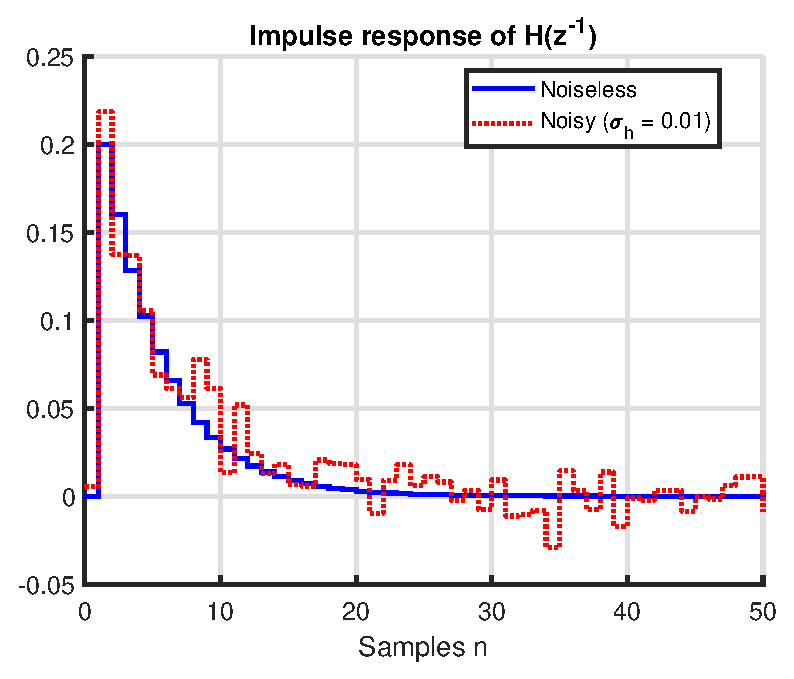
\includegraphics[width = 0.65 \textwidth]{figures/parseval_signal.eps}
    \caption{Impulse response of (\ref{eq:parseval_example_H}) with and without additive Gaussian white noise.}
    \label{fig:parseval_signal}
\end{figure}

The approximate cost function of the signal in the TD $\frac{1}{51^2}\sum_{n=0}^{l_1} h(n,\rho)^2$ is plotted in figure \ref{fig:parseval_energy} (blue full line). It quickly converges to the cost function of the signal in the FD $\frac{1}{51} \sum_{k=0}^{50} |H(k)|^2$. This is also the case for the noisy signal (dotted red line); it converges to its cost in the FD. Ideally however, we would like the cost in the noisy case to be as close to the actual, noiseless cost. This is not the case; there is a certain bias. In this case, taking $l_1 = 10$, would result in less bias, while still keeping the information that is needed. This can also be seen in figure \ref{fig:parseval_signal}: the impulse response after $n = 10$ is at or below noise level. Thus the impulse response after $n = 10$ does not contain much useful information and will only contribute to a biased cost.

\begin{figure}[H]
    \centering
    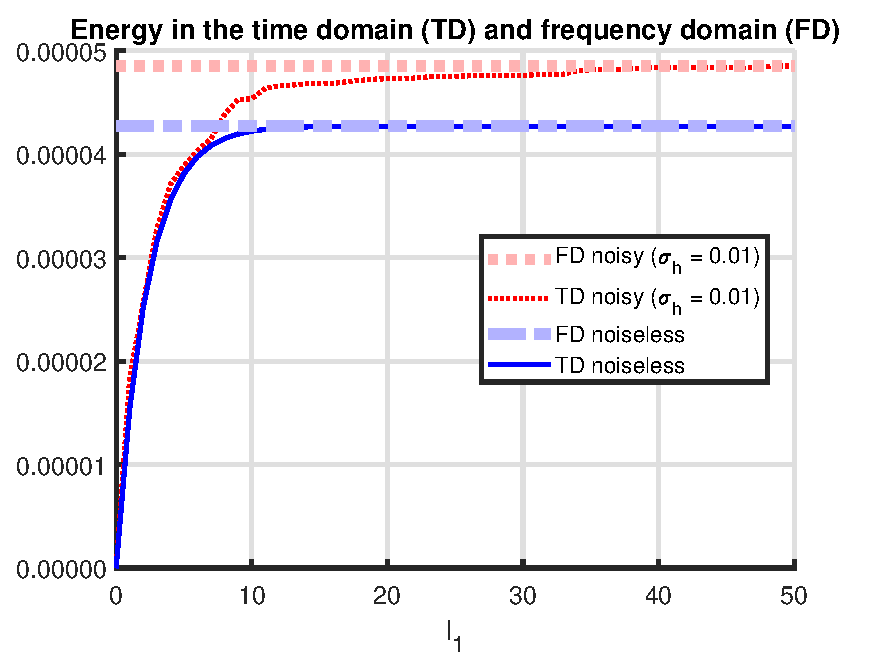
\includegraphics[width = 0.65 \textwidth]{figures/parseval_energy.eps}
    \caption{Energy of the signal in the TD and the FD (divided by $N$).}
    \label{fig:parseval_energy}
\end{figure}

In \cite{Data-driven_model_reference_control}, $l_1$ has a slightly different interpretation. As it can be seen in (\ref{eq:JNl1}), the sum goes from $-l_1$ to $l_1$. This is because the sum is taken over the cross-correlation of $u_W$ and $\epsilon$. The cross-correlation is meaningful for both positive and negative indices, which is why the sum also extends into negative values of $\tau$. The impulse response for negative indices is zero for causal systems, which is why the sum starts at $n = 0$ in (\ref{eq:Japprox_impulse_response}).

\newpage
\section{Bias}
\label{sec:bias}
Let's quantify the bias that was mentioned in the previous section. Let's assume that the input is a periodic signal that excites all the DFT frequencies. The output is perturbed by filtered white noise.
\begin{equation*}
    Y^{(p)}(k) = G(\Omega_k)U_0(k) + S_v(\Omega_k) V^{(p)}(k)
\end{equation*}
with $\mathbb{E}\{V^{(p)}(k)\} = 0$ and $\mathbb{E}\{|V^{(p)}(k)|^2\} = \sigma^2/N$. The nonparametric estimate of the FRF is
\begin{equation*}
    \hat G(\Omega_k) = \frac{\frac{1}{P}\sum_{p=0}^{P-1}  Y^{(p)}(k)}{\frac{1}{P}\sum_{p=0}^{P-1}  U^{(p)}(k)} = G(\Omega_k) + \frac{1}{U_0(k)} \frac{1}{P}\sum_{p=0}^{P-1} S_v(\Omega_k) V^{(p)}(k)
\end{equation*}
The statistical properties of this estimator are
\begin{align*}
    \mathbb{E}\{\hat G(\Omega_k)\} &= G(\Omega_k)\\
    \mathrm{Var}\{|\hat G(\Omega_k)|\} &= \frac{1}{N\!P}\frac{|S_v(\Omega_k)|^2 \sigma^2}{|U_0(k)|^2}
\end{align*}
$|S_v(\Omega_k)|^2 \sigma^2$ quantifies the power of the noise at the $k$-th DFT bin and $|U_0(k)|^2$ quantifies the energy of the signal at the $k$-th bin. This becomes evident when the RMS of the signals is calculated.
\begin{equation*}
    \text{RMS} = \sqrt{\frac{1}{N}\sum_{n=0}^{N-1} x(n)^2} = \sqrt{\sum_{k=0}^{N-1} |X(k)|^2}
\end{equation*}
Thus, $\frac{|S_v(\Omega_k)|^2 \sigma^2}{|U_0(k)|^2}$ is the noise-to-signal ratio at the $k$-th DFT bin.

Now we have the information we need to calculate the expected value of the cost function.
\begin{equation*}
    J_N(\rho) = \frac{1}{N}\sum_{k=0}^{N-1} |H(\Omega_k,\rho)|^2 = \frac{1}{N} \sum_{k=0}^{N-1} \Bigg|F(\Omega_k)(1-M(\Omega_k)) \Big[M(\Omega_k)-(1-M(\Omega_k))K(\Omega_k,\rho) \hat{G}(\Omega_k)\Big]\Bigg|^2
\end{equation*}
Taking the expected value gives
\begin{align*}
    \mathbb{E}\{J_N(\rho)\} &= \frac{1}{N}\sum_{k=0}^{N-1} \Bigg|F(\Omega_k)(1-M(\Omega_k)) \Big[M(\Omega_k)-(1-M(\Omega_k))K(\Omega_k,\rho) G(\Omega_k)\Big]\Bigg|^2 \\
    &+ \frac{1}{N} \sum_{k=0}^{N-1} \frac{1}{N\!P} \frac{|S_v(\Omega_k)|^2 \sigma^2}{|U_0(k)|^2} \Bigg|F(\Omega_k)(1-M(\Omega_k))^2 K(\Omega_k,\rho) \Bigg|^2  \\
    &= \Tilde{J}_N(\rho) + \frac{\sigma^2}{N^2 P} \sum_{k=0}^{N-1} \frac{|F(\Omega_k)|^2|1-M(\Omega_k)|^4 |K(\Omega_k,\rho)|^2}{\text{SNR}(k)}
\end{align*}
with $\Tilde{J}_N(\rho)$ being the cost function in the noiseless case and $\text{SNR}(k) = \frac{|U_0(k)|^2}{|S_v(\Omega_k)|^2 \sigma^2}$. So, it has been shown that the expected value of the cost function in the noisy case is not equal to the noiseless cost function. This is not a problem if the second term does not depend on $\rho$, as the optimization parameters that minimize $\mathbb{E}\{J_N(\rho)\}$ would also minimize $\Tilde{J}_N(\rho)$. However, in this case the second term does depend on $\rho$, which is the cause of the noise induced bias.

What if we now transform $H(\Omega_k,\rho)$ to the TD using the IDFT and approximate the cost function by only summing till $l_1$?
\begin{equation*}
    J_N(\rho) = \frac{1}{N} \sum_{k=0}^{N-1} |H(\Omega_k,\rho)|^2 = \frac{1}{N^2}\sum_{n=0}^{N-1} h(n,\rho)^2 \approx  \frac{1}{N^2}\sum_{n=0}^{l_1} h(n,\rho)^2 = J_{N,l_1}(\rho)
\end{equation*}
Because the sum only contains $(l_1+1)$ noisy terms, the bias will be smaller compared with the full sum. To be more specific, the bias will be a factor $(l_1+1)/N$ smaller. Thus the expected value of the approximate cost function becomes
\begin{equation}
\boxed{
    \mathbb{E}\{J_{N,l_1}(\rho)\} \approx \Tilde{J}_N(\rho) +  \frac{\sigma^2}{N^2 P} \frac{l_1+1}{N} \sum_{k=0}^{N-1} \frac{|F(\Omega_k)|^2|1-M(\Omega_k)|^4 |K(\Omega_k,\rho)|^2}{\text{SNR}(k)}
    }
    \label{eq:EJl1_FD}
\end{equation}
Thus, the bias can be decreased by only taking the first $l_1+1$  terms in the TD. However, making $l_1$ too small will invalidate the approximation $J_N(\rho) \approx J_{N,l_1}(\rho)$. Additionally, the bias can also be decreased by increasing the number of periods $P$, increasing the number of samples per period $N$ or by increasing the signal-to-noise ratio $\textrm{SNR}(k)$.

\section{Weighted nonlinear least squares}
\label{sec:WNLS}
It is possible to reduce the variability by using a weighted cost function. The weights will be based on the variance of the FRF estimate.
\begin{align*}
    \sigma^2_{\hat G}(\Omega_k) = \mathbb{E}\big\{|\hat G(\Omega_k)- \mathbb{E}\{\hat G(\Omega_k)\}|^2\big\} 
\end{align*}
The robust LPM can estimate the variance of the FRF estimate $\hat\sigma^2_{\hat G}$ for systems excited by periodic inputs. The weighted nonlinear least squares cost function is
\begin{equation}
\boxed{
    J_\mathrm{WNLS}(\rho) = \frac{1}{|\kexc|}\sum_{k \in \kexc} \frac{|H(\Omega_k,\rho)|^2}{\hat\sigma^2_{H}(\Omega_k,\rho)}}
    \label{eq:JWNLS}
\end{equation}
with $\kexc$ being the set of excited DFT bins and
\begin{equation*}
    H(\Omega_k,\rho) = F(\Omega_k)(1-M(\Omega_k)) \Big[M(\Omega_k)-(1-M(\Omega_k))K(\Omega_k,\rho) \hat{G}(\Omega_k)\Big]
\end{equation*}
and
\begin{equation*}
\hat\sigma^2_{H}(\Omega_k,\rho) = \hat\sigma^2_{\hat G}(\Omega_k) \Big| F(\Omega_k) (1-M(\Omega_k))^2K(\Omega_k,\rho) \Big|^2
\end{equation*}


The expected value of (\ref{eq:JWNLS}) is
\begin{align*}
\mathbb{E}\{J_\mathrm{WNLS}(\rho)\} &=
 \frac{1}{|\kexc|} \sum_{k \in \kexc} \frac{|F(1-M)|^2 |M-(1-M)K(\rho)G|^2}{|F(1-M)^2 K(\rho)|^2 \hat\sigma^2_{\hat G}}\\ 
 &+ \frac{1}{|\kexc|} \sum_{k \in \kexc} \frac{|F(1-M)^2 K(\rho)|^2 \sigma^2_{\hat G}}{|F(1-M)^2 K(\rho)|^2 \hat\sigma^2_{\hat G}} \\
&=  \Tilde{J}_\mathrm{WNLS}(\rho) + \frac{1}{|\kexc|} \sum_{k \in \kexc} \frac{\sigma^2_{\hat G}(\Omega_k)}{\hat\sigma^2_{\hat G}(\Omega_k)} 
\end{align*}
with $\Tilde{J}_\mathrm{WNLS}(\rho)$ being the cost function when $G(\Omega_k)$ is known exactly. The frequencies $\Omega_k$ are left out in the first equation for simplicity. The second term does not depend on $\rho$, which means that the optimization parameters $\rho$ that minimize $\mathbb{E}\{J_\mathrm{WNLS}(\rho)\}$ will also minimize $\Tilde{J}_\mathrm{WNLS}(\rho)$. After all, the second term is just a constant independent of $\rho$.


\paragraph{Realizable ideal controller}
If the ideal controller is realizable, then
\begin{equation*}
\Tilde{J}_\mathrm{WNLS}(\rho^*) = 0
\end{equation*}
The convex cost function (\ref{eq:JFD}) is also zero in $\rho = \rho^*$ in the noiseless case. This means that the original cost function (\ref{eq:Jmr}), the convex cost function (\ref{eq:J}) and the WNLS cost function (\ref{eq:JWNLS}) are all minimal in $\rho = \rho^*$. Therefore, if the ideal controller is realizable, then the WNLS optimization has the potential to give a better estimate of the ideal controller as the WNLS cost function also takes the noise variance into account.


\paragraph{Non realizable ideal controller}
On the other, what happens if the ideal controller is not realizable? In this case, the minimum of any of the costs will be greater than 0, even in the noiseless case. Thus, the optimization parameters $\rho$ that minimize the original cost function, the convex cost function and the WNLS cost function will be different in general.


\paragraph{Optimization strategy}
The cost function (\ref{eq:JWNLS}) is not convex any more as the denominator also depends on the optimization parameters $\rho$. Thus, the minimization of this cost function cannot be solved with convex optimization. It can be solved with the Gauss-Newton algorithm. An initial estimate of $\rho$ can be found by minimizing the convex cost function (\ref{eq:JFD}). The danger however, is that this optimization might not converge to the global minimum.


\section{Summary}
The steps that must be taken in order to find a controller using model reference control are summarized in figure \ref{fig:flowchart}. Measurements of the (noisy) SISO system are given. These are necessary for the optimization.
%Note that the output is assumed to be perturbed by filtered white noise with noise model $S_y(q^{-1})$. However, the input can also be noisy and the different optimization strategies also work when this is the case. Moreover, no system is LTI in the real world. Nevertheless, it is still useful to assume that they are.

%Measurements of the system input and output are necessary for the optimization. 

The user must then also define the reference model $M(\Omega)$ and the controller structure $K(\Omega,\rho)$. Then, the user can choose one of the optimization criteria that were discussed in the previous sections. This results in the optimal parameters $\rho_{\mathrm{opt}}$, from which the optimal controller $K(\Omega,\rho_{\mathrm{opt}})$ can be determined.

\begin{figure}[H]
\centering
\includegraphics[width = 0.75\textwidth]{figures/flowchart.pdf}
\caption{Flowchart of the steps taken in model reference control.}
\label{fig:flowchart}
\end{figure}


\newpage
\section{Discrete-time simulations}
\label{sec:DT_simulations}

\subsection{Introduction}
\label{sec:DT_simulations_introduction}
First, an important approximation was made in the previous sections. Initially, it was assumed that the sensitivity function can be approximated by the ideal sensitivity function.
\begin{equation*}
\frac{1}{1 + K(\Omega,\rho) G(\Omega)} \approx \frac{1}{1 + K^{*}(\Omega) G(\Omega)}
\end{equation*}
This was done in order to make the cost function convex. Thus we should verify after optimization that the original cost function (\ref{eq:Jmr}) can be approximated by the convex cost function (\ref{eq:J}).
\begin{equation*}
	J_{mr}(\rho) \approx J(\rho)
\end{equation*}

\paragraph{System models}
In order to compare the FD methods to the TD methods, we will initially work with DT systems. 3 DT systems $G(q^{-1})$ will be simulated. The first 2 systems will have a reference model $M(q^{-1})$ that will be realizable by the proposed control structure $K(q^{-1},\rho)$. The third system will have a reference model that cannot be realized by the proposed control structure. The systems, the reference models and the proposed controller structures are given in table \ref{tab:simulated_systems}. These are also shown in figure \ref{fig:G_and_M_all}. The systems will start with zero initial conditions.

\begin{table}[H]
\centering
\begin{tabular}{|ccc|}
\hline
Name & Simple system & Long transient system\\
\hline
&&\\[-2.5ex]
$G(q^{-1})$ & $\dfrac{0.25 q^{-1}}{1 - 0.75 q^{-1}}$ & $\dfrac{1.785 q^{-1} + 1.701 q^{-2}}{1 + 1.558 q^{-1} + 0.9274 q^{-2}}$ \\
\hline
&&\\[-2.5ex]
$M(q^{-1})$ & $\dfrac{0.15 q^{-1} - 0.075 q^{-2}}{1 - 1.6 q^{-1} + 0.675 q^{-2}}$ & $\dfrac{0.1785 q^{-1} + 0.3486 q^{-2} + 0.1701 q^{-3}}{1 + 0.7369 q^{-1} - 0.2824 q^{-2} - 0.7573 q^{-3}}$ \\
\hline
&&\\[-2.5ex]
$K(\rho,q^{-1})$ & $\dfrac{\rho_0 + \rho_1 q^{-1}}{1-q^{-1}}$ & $\dfrac{\rho_0 + \rho_1 q^{-1}}{1-q^{-1}}$ \\
\hline
Realizable & Yes & Yes \\
\hline
\hline
Name & \multicolumn{2}{c|}{System with non realizable controller} \\
\hline
&&\\[-2.5ex]
$G(q^{-1})$ & \multicolumn{2}{c|}{$\dfrac{0.7893 q^{-3}}{1 - 1.418 q^{-1} + 1.59 q^{-2} - 1.316 q{^-3} + 0.886 q^{-4}}$}\\
\hline
&&\\[-2.5ex]
$M(q^{-1})$ & \multicolumn{2}{c|}{$\dfrac{0.1552 q^{-3}}{1 - 1.212 q^{-1} + 0.3672 q^{-2}}$} \\
\hline
&&\\[-2.5ex]
$K(\rho,q^{-1})$ & \multicolumn{2}{c|}{$\dfrac{\rho_0 + \rho_1 q^{-1} + \rho_2 q^{-2} + \rho_3 q^{-3} + \rho_4 q^{-4}}{1-q^{-1}}$} \\
\hline
Realizable & \multicolumn{2}{c|}{No} \\
\hline
\end{tabular}
\caption{Simulated system and the reference models.}
\label{tab:simulated_systems}
\end{table}


\begin{figure}[H]
\centering
\begin{subfigure}{.33\textwidth}
	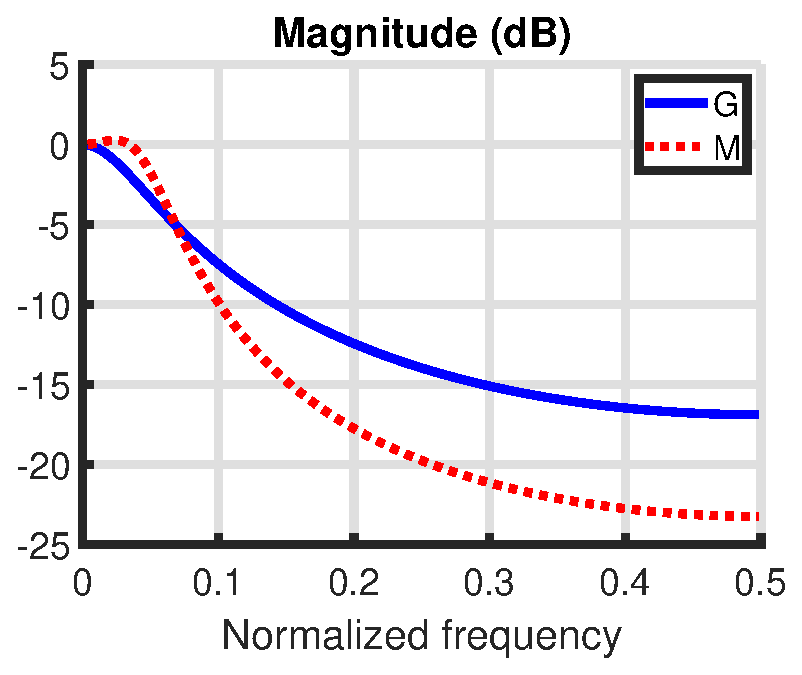
\includegraphics[width=\linewidth]{figures/G_and_M_simple.eps}
	\caption{Simple system}
\end{subfigure}%
\begin{subfigure}{.33\textwidth}
	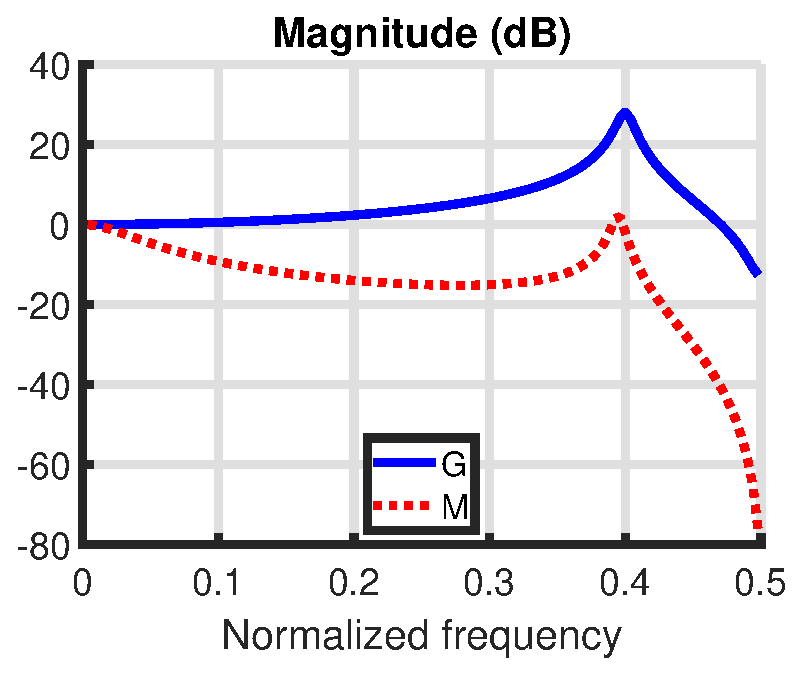
\includegraphics[width=\linewidth]{figures/G_and_M_long_transient.eps}
	\caption{Long transient system}
\end{subfigure}%
\begin{subfigure}{.33\textwidth}
	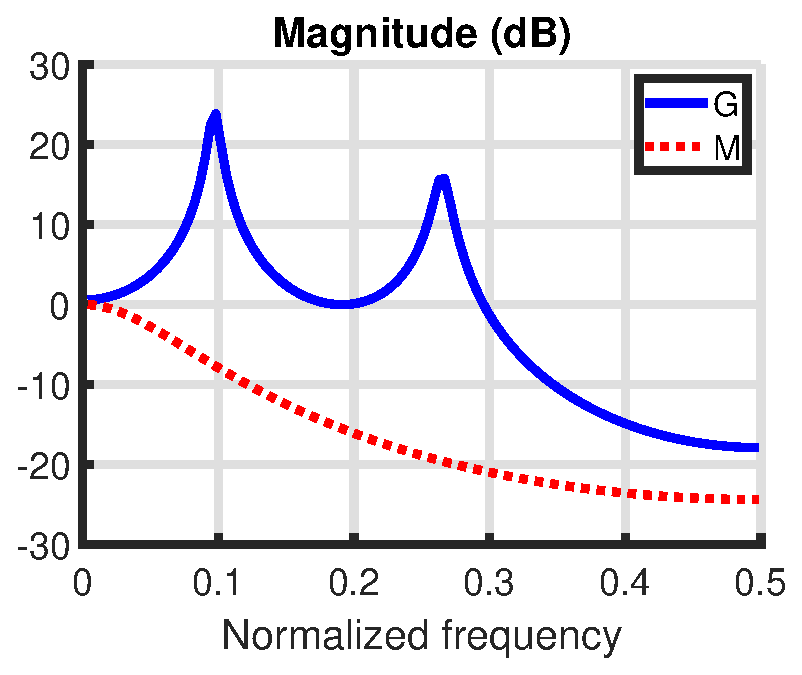
\includegraphics[width=\linewidth]{figures/G_and_M_undermodeled.eps}
	\caption{System with non realizable controller}
\end{subfigure}
\caption{Magnitude bode plots of the system and the reference models.}
\label{fig:G_and_M_all}
\end{figure}

\paragraph{Noise models}
The output of the systems will be perturbed by DT filtered Gaussian white noise.
\begin{equation*}
	y(n) = G(q^{-1}) u(n) + S_y(q^{-1}) e(n) \text{ with } e(n) \sim \mathcal{N}(0,\sigma^2)
\end{equation*}

2 different noise models will be used:
\begin{itemize}
\item $S_y(q^{-1}) = 1$, i.e white noise 
\item $S_y(q^{-1}) = \dfrac{0.1105 q^{-1} - 0.06831 q^{-2} + 0.04222 q^{-3} + 0.04222 q^{-3} - 0.06831 q^{-4} + 0.1105 q^{-5}}{1 - 0.3337 q^{-1} - 0.3872 q^{-2} - 0.1103 q^{-3}}$
\end{itemize}
The magnitude bode plots of the noise models are shown in figure \ref{fig:noise_models}. For every simulation the noise standard deviation is set to $\sigma = 0.2$.

\begin{figure}[H]
\centering
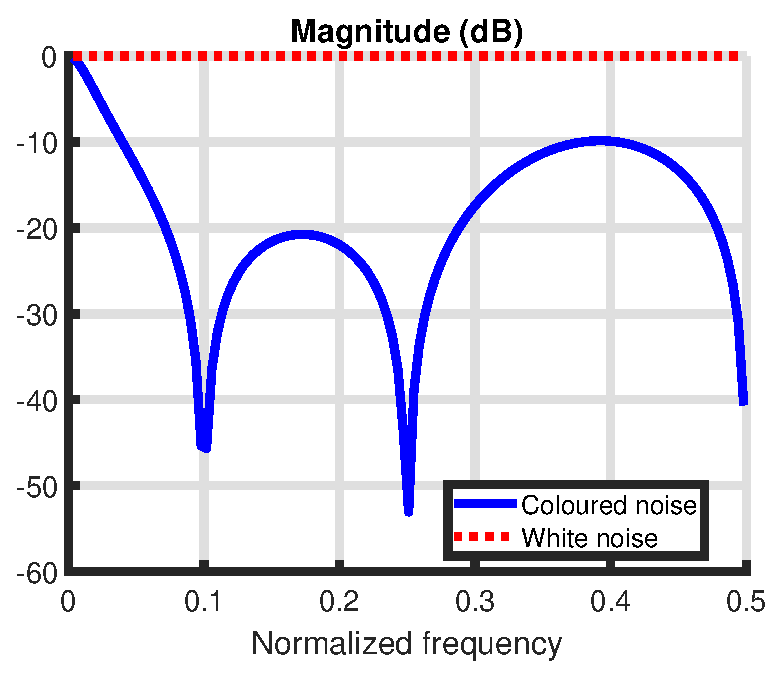
\includegraphics[width=0.6\linewidth]{figures/noise_models.eps}
\caption{Magnitude bode plots of the noise models.}
\label{fig:noise_models}
\end{figure}

\paragraph{Optimization strategies}
As explained in the previous sections, there are multiple ways to find the optimal controller. 

First, the optimal $\rho$ for a certain frequency resolution $f_s/N$ can be found by minimizing $(\ref{eq:JFD})$ and by replacing $\hat{G}(\Omega_k)$ with the actual system $G(\Omega_k)$. This can be done because we are working in a simulation. Note however, that we are optimizing the convex cost function. If the reference model $M$ is realizable, then $J_{mr}(\rho^*) = J(\rho^*) = 0$, which means that, in the noiseless case, the parameters $\rho$ that minimize the convex cost function will also minimize the original cost function. This is not the case any more if the reference model is not realizable.

The TD method consists of minimizing (\ref{eq:JNl1}) w.r.t. $\rho$. However, the parameter $l_1$ must be chosen by the user. The maximum value that can be chosen for $l_1$ is $N/2$. 

The FD method consists of minimizing (\ref{eq:JFD}) w.r.t. $\rho$. The $l_1$-trick can also be used here by minimizing 
\begin{equation}
\boxed{
J_{N,l_1}(\rho) = \frac{1}{N^2}\sum_{n=0}^{l_1} h(n,\rho)^2}
\label{eq:JNl1_FD}
\end{equation}
with $h(n,\rho)$ being the IDFT of $H(\Omega_k,\rho)$. Notice that when $l_1 = N - 1$, $J_{N,l_1}(\rho) = J_N(\rho)$ in the FD.

Finally, the WNLS method will also be used by minimizing (\ref{eq:JWNLS}). This cost function will be minimized by using the Gauss-Newton algorithm. The maximum number of iterations is set to 100 and the algorithm is stopped if the relative difference between the previous and the next estimate is smaller than $10^{-10}$ for all $\rho_i$ in $\rho$. An initial estimate for $\rho$ is found by using the FD method with $l_1 = N-1$. As there is no guarantee that this optimization will converge to the global minimum, the optimization will also be started at the optimal $\rho$ for comparison. Of course, this can only be done because we are working in a simulation.


\paragraph{Input}
The input will be a random phase multisine where all harmonics are excited. The RMS of this multisine is 1 and it is repeated for $P=4$ periods. None of the periods are discarded. The number of samples per period is $N=255$. 

\paragraph{Nonparametric estimate}
The FD methods require a nonparametric estimate. Two different nonparametric estimates are used. The first one is without any removal of system and noise transients by using (\ref{eq:nonparametric_simple}). The second way of obtaining a nonparametric estimate is by using the robust LPM with order $R=2$ and degrees of freedom $q^{\mathrm{noise}}=1$. These values were obtained by using the heuristics mentioned in section \ref{sec:choice_order_dof}. Finally, the WNLS method needs the variance of the FRF estimate. This is also obtained via the robust LPM.

\paragraph{Evaluation}
100 noise realizations are simulated. The resulting controllers are compared by evaluating the cost function with the real system $G(\Omega)$. Both the original cost function and the convex cost function are calculated.
\begin{align*}
J_{mr}(\rho) &= \frac{1}{127} \sum_{k=1}^{127} \Big|M(\Omega_k) - \frac{K(\Omega_k,\rho)G(\Omega_k)}{1+K(\Omega_k,\rho)G(\Omega_k)}\Big|^2\\
J(\rho) &= \frac{1}{127} \sum_{k=1}^{127} \Big|(1-M(\Omega_k))\big[M(\Omega_k) - (1-M(\Omega_k))K(\Omega_k,\rho)G(\Omega_k)\big]\Big|^2
\end{align*}
where $\rho$ is obtained by optimization for one noise realization with any of the methods. Note that $F(\Omega_k)=1$ in the above equations. The sum starts at 1 because DC is not excited by the input. The sum ends at 127 because there are 127 excited harmonics in the input. Then the cost of the controllers obtained from the different noise realizations can be averaged.
\begin{align*}
\Bar{J}_{mr} &= \frac{1}{100} \sum_{i=1}^{100} J_{mr}(\rho^{(i)})\\
\Bar{J} &= \frac{1}{100} \sum_{i=1}^{100} J(\rho^{(i)})
\end{align*}
where $\rho^{(i)}$ are the parameters obtained by optimizing the cost corresponding to the \mbox{$i$-th} noise realization with one of the optimization methods. Note that TD methods with different values of $l_1$ are considered different and shouldn't be mixed up when taking the mean. Finally, the mean cost function can be expressed in decibels.
\begin{align*}
\Bar{J}_{mr}|_{dB} &= 10 \log_{10}(\Bar{J}_{mr}) \\
\Bar{J}|_{dB} &= 10 \log_{10}(\Bar{J})
\end{align*}

\newpage

\subsection{Simple system}
\paragraph{Influence of $\mathbf{l_1}$}
Let's start by seeing how the choice of $l_1$ influences the performance of the resulting controller. The simple system is simulated with disturbing white output noise as explained above. For the TD method, all values of $l_1$  between 1 and $\lfloor N/2 \rfloor = 127$ are tried for each noise realization. For the FD method, all values of $l_1$ between 1 and $N-1 = 254$ are tried for each noise realization. 
The resulting closed loop systems that are obtained by applying the FD method with $l_1 = 1,17  \text{ and } 254$ are shown in figure \ref{fig:CL_FD_simple_flat}. The closed loop system resulting from $l_1=1$ performs poorly and doesn't get close to the reference model $M$. The result is better when $l_1 = 254$, but is best when $l_1 = 17$.

\begin{figure}[H]
\centering
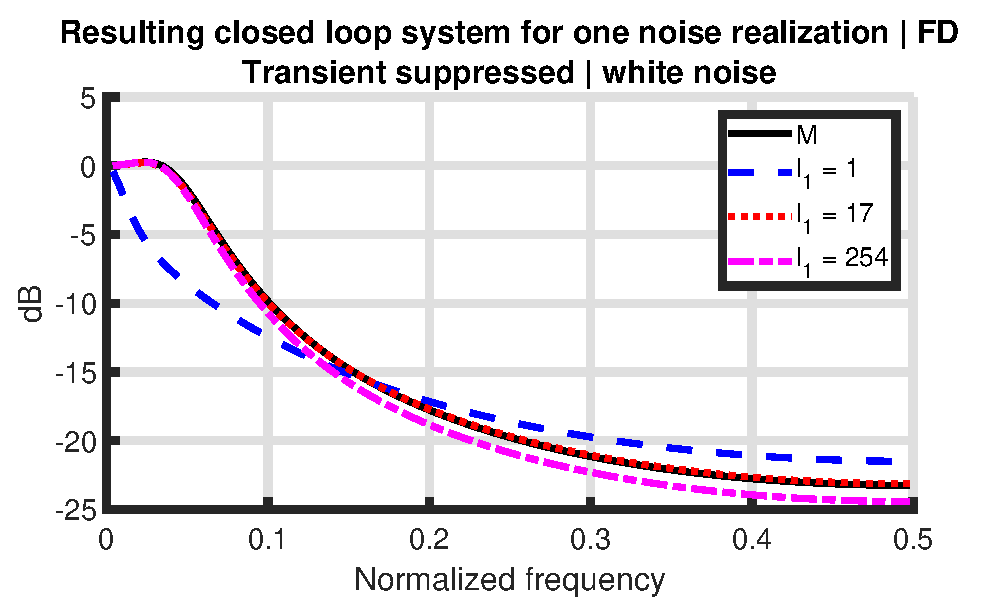
\includegraphics[width=0.6\textwidth]{figures/CL_FD_simple_flat.eps}
\caption{Resulting CL systems for one white noise realization by applying the FD method with different values of $l_1$.}
\label{fig:CL_FD_simple_flat}
\end{figure}

\newpage
The mean cost function for the TD and FD methods for different values of $l_1$ are shown in figure \ref{fig:mean_cost_function_simple_flat}. The mean cost function has a bowl shape as a function of $l_1$. This is because too much information is thrown away when taking a too small $l_1$. However, taking a large $l_1$ just increases the bias. This was also observed in the figure \ref{fig:CL_FD_simple_flat}. One more thing to note is that the original cost function $J_{mr}$ coincides with the convex cost function $J$ most of the time. This means that the sensitivity function can be approximated quite well by the ideal sensitivity function. The cost functions don't coincide for the FD method when $l_1=1$. This is because the resulting closed loop system doesn't come very close to the reference model $M$, as can be seen figure \ref{fig:CL_FD_simple_flat}.

\begin{figure}[H]
\centering
\begin{subfigure}{0.6\textwidth}
	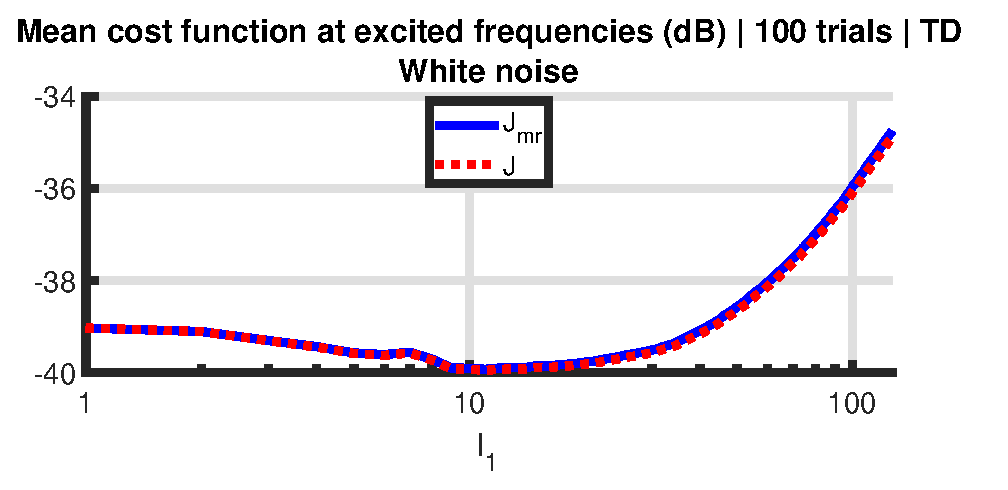
\includegraphics[width=\linewidth]{figures/mean_cost_function_TD_simple_flat.eps}
	\caption{TD method for different $l_1$.}
\end{subfigure}

\begin{subfigure}{0.6\textwidth}
	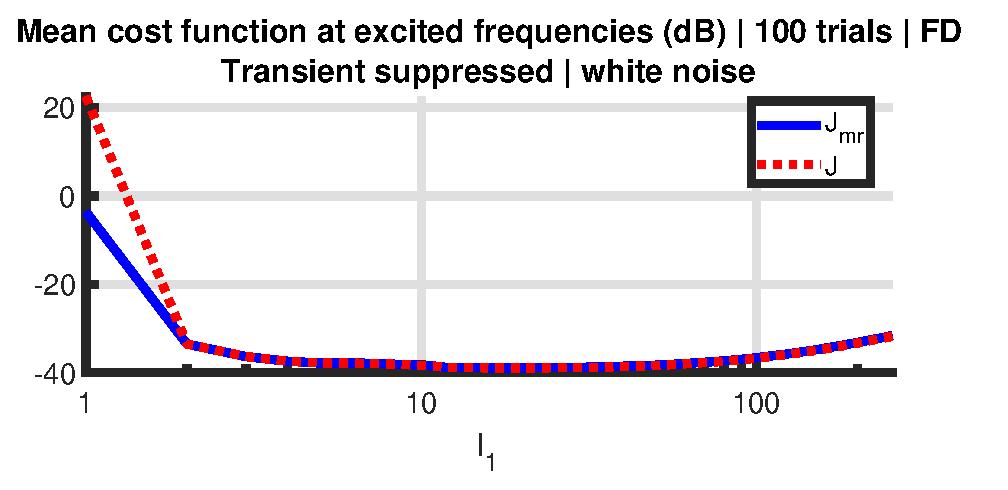
\includegraphics[width=\linewidth]{figures/mean_cost_function_FD_simple_flat.eps}
	\caption{FD method for different $l_1$ and suppression of the transient.}
\end{subfigure}
\caption{Mean cost functions for 100 noise realizations, applied to the simple system with a white noise model.}
\label{fig:mean_cost_function_simple_flat}
\end{figure}

\paragraph{Transient suppression}
In the previous experiment, the transient was suppressed by using the robust LPM. What will happen if the transient is not suppressed? The mean cost function obtained when applying the FD methods with $l_1=254$ with and without transient suppression are given in table \ref{tab:simple_flat_FD_transient_with_without}. Not suppressing the transient gives better results. This is to be expected as the simple system has a very low transient. Moreover, there are no noise transients because the noise is white.
    
\begin{table}[H]
\centering
\begin{tabular}{|ccc|}
\hline
&&\\[-2.5ex]
Method & $\Bar{J}|_{dB}$ & $\Bar{J_{mr}}|_{dB}$ \\
\hline
Transient suppressed & -31.74 & -31.57\\
Transient not suppressed & \textbf{-34.86} & \textbf{-34.73}\\
\hline
\end{tabular}
\caption{FD method with $l_1= 254$ applied to simple system with white noise. With and without transient suppression.}
\label{tab:simple_flat_FD_transient_with_without}
\end{table}

\newpage
Let's see what happens when the output is disturbed by coloured noise. The results of the same experiment, but with coloured noise are shown in table \ref{tab:simple_cololoured_FD_transient_with_without}. The results for coloured noise are better than the results for white noise (table \ref{tab:simple_flat_FD_transient_with_without}). However, this is an unfair comparison as the SNR is not the same in both experiments (see figure \ref{fig:noise_models}). This time, not suppressing the transient is still better.

\begin{table}[H]
\centering
\begin{tabular}{|ccc|}
\hline
&&\\[-2.5ex]
Method & $\Bar{J}|_{dB}$ & $\Bar{J_{mr}}|_{dB}$ \\
\hline
Transient suppressed & -50.99 &-50.98\\
Transient not suppressed & \textbf{-52.51} & \textbf{-52.52}\\
\hline
\end{tabular}
\caption{FD method with $l_1= 254$ applied to simple system with coloured noise. With and without transient suppression.}
\label{tab:simple_cololoured_FD_transient_with_without}
\end{table}


To see why this is the case, we can look at the mean squared error (MSE) of the nonparametric estimate of the transfer function over all the noise realizations. This is plotted in figure \ref{fig:MSE_Gest_simple_coloured}. The estimate with transient removal is better around the transmission zeros of the noise model. To understand why this is so, let's assume that the noise model is given by
\begin{equation*}
	S_y(q^{-1}) = \frac{C(q^{-1})}{D(q^{-1})}
\end{equation*}
In that case, the contribution of the noise on the output at the $k$-th bin is
\begin{equation*}
	\frac{C(\Omega_k)}{D(\Omega_k)} E(k) + \frac{I_E(\Omega_k)}{D(\Omega_k)} = \frac{C(\Omega_k) E(k) + I_E(\Omega_k)}{D(\Omega_k)}
\end{equation*}
with $E(k)$ being the DFT of $e(n)$ and $I_E(\Omega_k)$ being a polynomial in $\Omega_k$ that depends on the initial and end conditions of $e(n)$. When $C(\Omega_k)$ is small, the contribution of the noise is mainly attributed to the transient term $\frac{I_E(\Omega_k)}{D(\Omega_k)}$. Thus, the transient term is dominant at transmission zeros of the noise model. However, at the other frequencies where the random term $\frac{C(\Omega_k)}{D(\Omega_k)} E(k)$ is dominant, the estimate of the FRF is slightly worse (around 1 dB) when taking the transient into account. As the optimization takes all the frequency bins into account, an improvement around the transmission zeros is not enough to improve the estimate of the optimal controller in this case.

\begin{figure}[H]
\centering
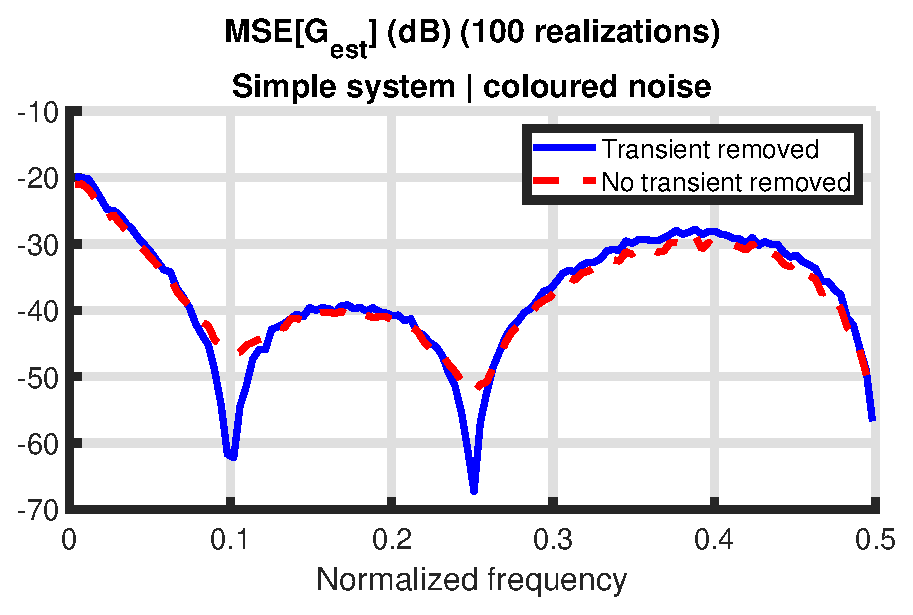
\includegraphics[width=0.6\textwidth]{figures/MSE_Gest_simple_coloured.eps}
\caption{MSE error of the nonparametric estimate of the simple system in the presence of coloured noise with and without transient suppression.}
\label{fig:MSE_Gest_simple_coloured}
\end{figure}

\newpage
\paragraph{TD vs. FD vs. WNLS}
Let's now compare the TD, FD and WNLS methods. For the FD method, the transient can be either suppressed or not taken into account. The WNLS method also uses a nonparametric estimate of the FRF, so here the transient can also be suppressed or not taken into account. Additionally, this optimization needs an initial estimate. As we are working in simulation, the actual parameters $\rho$ that minimize the convex cost function are known. If these parameters are used as initial estimate, we refer to this optimization as ``actual init''. If the estimate of the controller parameters obtained by optimizing using the FD method with $l_1 = 254$ are used as initial estimate, then we refer to this optimization as ``LS init''. The reason for referring to this initial estimate as ``LS init'' is because it is obtained by minimizing the numerator of (\ref{eq:JWNLS}), which is equivalent to minimizing (\ref{eq:JFD}). The numerator of (\ref{eq:JWNLS}) is the sum of squares, which is why the result of this optimization is referred to as the least squares (LS) solution. Table \ref{tab:simple_white_transient_with_without_TD_vs_FD_vs_WNLS} compares the mean cost function of all the methods on the simple system with additive white noise. For the first 3 rows, the parameters $l_1$ that performs the best are shown. The FD method with $l_1 = 23$ where the transient is not suppressed performs best. Moreover, the WNLS method achieves exactly the same results when using the ``LS init'' or the ``actual init''. This means that the ``LS init'' is a good initial estimate for the optimization.

\begin{table}[H]
\centering
\begin{tabular}{|ccc|}
\hline
&&\\[-2.5ex]
Method & $\Bar{J}|_{dB}$ & $\Bar{J_{mr}}|_{dB}$ \\
\hline
TD ($l_1 = 11$) & -39.95 & -39.92 \\
FD transient not suppressed ($l_1 = 23$) & \textbf{-40.03} & \textbf{-40.01} \\
FD transient suppressed ($l_1 = 17$) & -38.95 & -38.92 \\
WNLS transient not suppressed (LS init) & -37.25 & -37.34 \\
WNLS transient not suppressed (actual init) & -37.25 & -37.34 \\
WNLS transient suppressed (LS init) & -37.96 & -37.96 \\
WNLS transient suppressed (actual init) & -37.96 & -37.96 \\
\hline
\end{tabular}
\caption{Simple system with white noise. With and without transient suppression for the FD and WNLS methods. For the first 3 rows, the parameters $l_1$ that yielded the best results are displayed.}
\label{tab:simple_white_transient_with_without_TD_vs_FD_vs_WNLS}
\end{table}

Table \ref{tab:simple_white_transient_with_without_TD_vs_FD_vs_WNLS} showed the results for additive white noise. What will happen if the output is perturbed by coloured noise?  The results for this experiment are shown in table \ref{tab:simple_coloured_transient_with_without_TD_vs_FD_vs_WNLS}. The TD method now performs better than the FD method. However, the WNLS method outperforms the other methods in this case by a large margin. Additionally, even though the WNLS method without transient suppression is better than the other methods, the WNLS method with transient suppression gives a very large improvement. Also, using the ``LS init'' yields exactly the same result as using the ``actual init''.

\begin{table}[H]
\centering
\begin{tabular}{|ccc|}
\hline
&&\\[-2.5ex]
Method & $\Bar{J}|_{dB}$ & $\Bar{J_{mr}}|_{dB}$ \\
\hline
TD ($l_1 = 7$) & -53.46 & -53.46 \\
FD transient not suppressed ($l_1 = 12$) & -52.62 & -52.64 \\
FD transient suppressed ($l_1 = 12$) & -52.31 & -52.31 \\
WNLS transient not suppressed (LS init) & -57.04 & -57.04 \\
WNLS transient not suppressed (actual init) & -57.04 & -57.04 \\
WNLS transient suppressed (LS init) & \textbf{-69.64} & \textbf{-69.64} \\
WNLS transient suppressed (actual init) & \textbf{-69.64} & \textbf{-69.64} \\
\hline
\end{tabular}
\caption{Simple system with coloured noise. With and without transient suppression for the FD and WNLS methods. For the first 3 rows, the parameters $l_1$ that yielded the best results are displayed.}
\label{tab:simple_coloured_transient_with_without_TD_vs_FD_vs_WNLS}
\end{table}

\newpage
The reason why the WNLS method works better for coloured noise than for white noise is that the FRF estimate at all bins are equally noisy when the output is perturbed by white noise. Thus, using a weighting doesn't improve the quality of the controller. However, if the noise is highly coloured, the WNLS method will be more inclined to use the frequency bins where the noise is low to design a controller.

\subsection{Long transient system}
The long transient system is excited with the same signal as before (see section \ref{sec:DT_simulations_introduction}). The output is perturbed with additive white Gaussian noise. Again all values of $l_1$ between 1 and 127 are tried in the TD method and all values of $l_1$ between 1 and 254 are tried for the FD method. Additionally, the transient is either suppressed or not taken into account when estimating a nonparametric representation of the FRF. Finally, the WNLS method is also used to design the controller. A summary of the results is shown in table \ref{tab:long_transient_white_transient_with_without_TD_vs_FD_vs_WNLS}. In this case, the WNLS method with transient suppression gives the best results even though the output is perturbed by white noise. This wasn't the case for the simple system (table \ref{tab:simple_white_transient_with_without_TD_vs_FD_vs_WNLS}). 
%One thing to note is that the mean cost function is very high for the WNLS method where the transient is not suppressed with ``LS init'' as initial estimate. 
%This is because 1 of the 100 optimizations didn't converge to a minimum, causing the mean cost function to grow significantly.
One thing to note is that 1 of the 100 optimizations didn't converge to a minimum for the WNLS method where the transient is not suppressed with ``LS init'' as initial estimate. The failed optimization is not taken into account when calculating the mean cost function.
This shows that there is no guarantee of convergence to a global minimum when minimizing a non-convex cost function. Another interesting thing to note is that the FD method works better when the transient is suppressed, which wasn't the case for the simple system (tables \ref{tab:simple_white_transient_with_without_TD_vs_FD_vs_WNLS} and \ref{tab:simple_coloured_transient_with_without_TD_vs_FD_vs_WNLS}). This is expected as this system has a much longer transient than the simple system. Finally, the FD method with transient suppression achieves the best results when $l_1 = 102$. For the simple system the best results with the FD method were achieved with $l_1 = 23$ and $l_1 = 12$ for white and coloured noise respectively. This shows that more samples of the impulse response $h(n,\rho)$ are needed when the impulse response of the system $G(\Omega)$ is longer. In figure \ref{fig:impulse_simple_long} the impulse responses of the simple and the long transient systems are plotted. It is clear from this figure that $l_1$ should be taken bigger for the long transient system. 

\begin{table}[H]
\centering
\begin{tabular}{|ccc|}
\hline
&&\\[-2.5ex]
Method & $\Bar{J}|_{dB}$ & $\Bar{J_{mr}}|_{dB}$ \\
\hline
TD ($l_1 = 7$) & -54.06 & -54.06 \\
TD ($l_1 = 127$) &  -52.83 & -52.85 \\
FD transient not suppressed ($l_1 = 8$) & -46.71 & -46.66 \\
FD transient not suppressed ($l_1 = 254$) & -45.25 & -45.16 \\
FD transient suppressed ($l_1 = 102$) & -52.80 & -52.80 \\
FD transient suppressed ($l_1 = 254$) & -50.90 & -50.92 \\
WNLS transient not suppressed (LS init) & \textcolor{red}{-50.50 [1 failed]} & \textcolor{red}{-50.48 [1 failed]} \\
WNLS transient not suppressed (actual init) & -50.54 & -50.51 \\
WNLS transient suppressed (LS init) & \textbf{-59.10} & \textbf{-59.11} \\
WNLS transient suppressed (actual init) & \textbf{-59.10} & \textbf{-59.11} \\
\hline
\end{tabular}
\caption{Long transient system with white noise. With and without transient suppression for the FD and WNLS methods. For the first, third and fifth rows, the parameters $l_1$ that yielded the best results are displayed.}
\label{tab:long_transient_white_transient_with_without_TD_vs_FD_vs_WNLS}
\end{table}

\begin{figure}[H]
\centering
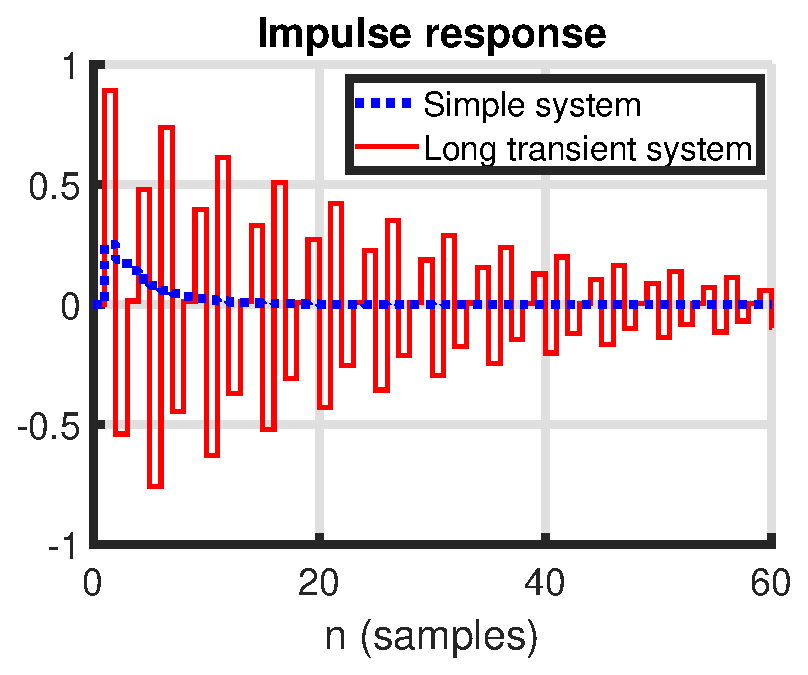
\includegraphics[width = 0.6\textwidth]{figures/impulse_response_simple_long}
\caption{Impulse response of the simple system and the long transient system.}
\label{fig:impulse_simple_long}
\end{figure}

The same experiment can be repeated with coloured noise. The summary of the results is shown in table \ref{tab:long_transient_coloured_transient_with_without_TD_vs_FD_vs_WNLS}. The same conclusions taken for the results of table \ref{tab:long_transient_white_transient_with_without_TD_vs_FD_vs_WNLS} can be applied here. One difference is that in this case, all the 100 optimizations failed for the WNLS method where the transient is not suppressed with ``LS init'' as initial estimate.
\begin{table}[H]
\centering
\begin{tabular}{|ccc|}
\hline
&&\\[-2.5ex]
Method & $\Bar{J}|_{dB}$ & $\Bar{J_{mr}}|_{dB}$ \\
\hline
TD ($l_1 = 2$) & -65.88 & -65.88 \\
TD ($l_1 = 127$) & -64.32 & -64.32 \\
FD transient not suppressed ($l_1 = 2$) & -50.83 & -50.81 \\
FD transient not suppressed ($l_1 = 254$) & -44.76 & -44.67 \\
FD transient suppressed ($l_1 = 133$) & -63.08 & -63.08 \\
FD transient suppressed ($l_1 = 254$) & -62.82 & -62.83 \\
WNLS transient not suppressed (LS init) & \textcolor{red}{[all failed]} & \textcolor{red}{[all failed]}   \\
WNLS transient not suppressed (actual init) & -64.71 & -64.71 \\
WNLS transient suppressed (LS init) & \textbf{-82.73} & \textbf{-82.73} \\
WNLS transient suppressed (actual init) & \textbf{-82.73} & \textbf{-82.73} \\
\hline
\end{tabular}
\caption{Long transient system with coloured noise. With and without transient suppression for the FD and WNLS methods. For the first, third and fifth rows, the parameters $l_1$ that yielded the best results are displayed.}
\label{tab:long_transient_coloured_transient_with_without_TD_vs_FD_vs_WNLS}
\end{table}

\newpage
\subsection{System with non realizable controller}
For the system with non realizable controller, the ideal controller $K^*(\Omega)$ cannot be realized by the proposed controller structure $K(\Omega,\rho)$. Thus, the cost function is strictly greater than 0 for any optimization parameter $\rho$. As was seen in section \ref{sec:WNLS}, this means that the original cost function, convex cost function and WNLS cost function will be minimized for different $\rho$, even in the noiseless case.

\paragraph{Optimal controller}
As we are working in simulation, the FRF of the system $G(\Omega)$ is known exactly. This knowledge can be used to get the optimal controller. The optimal controller was found by minimizing the convex cost function (\ref{eq:JFD}) while replacing the estimate of the FRF of the system $\hat{G}(\Omega_k)$ with the exact FRF of the system $G(\Omega_k)$. Note that the optimal controller will depend on the frequency resolution $f_s/N$ that the user chooses. In this case $N = 255$ as in the previous experiments. One could also minimize the original cost function (\ref{eq:Jmr}). However, we assume that the approximation made to attain the convex cost function is good enough to make little difference. The closed loop system resulting from the optimal controller is shown in figure \ref{fig:non_realizable_optimal}. If the ideal controller $K^*(\Omega)$ is realizable by the proposed controller structure $K(\Omega,\rho)$, then the closed loop system $\mathrm{CL}(\Omega)$ resulting from this noiseless optimization should be exactly equal to the reference system $M(\Omega)$. As the resulting closed loop system does not coincide with the reference model in the figure, it is evident that the reference system $M(\Omega)$ cannot be realized by the proposed controller structure $K(\Omega,\rho)$.

\begin{figure}[H]
\centering
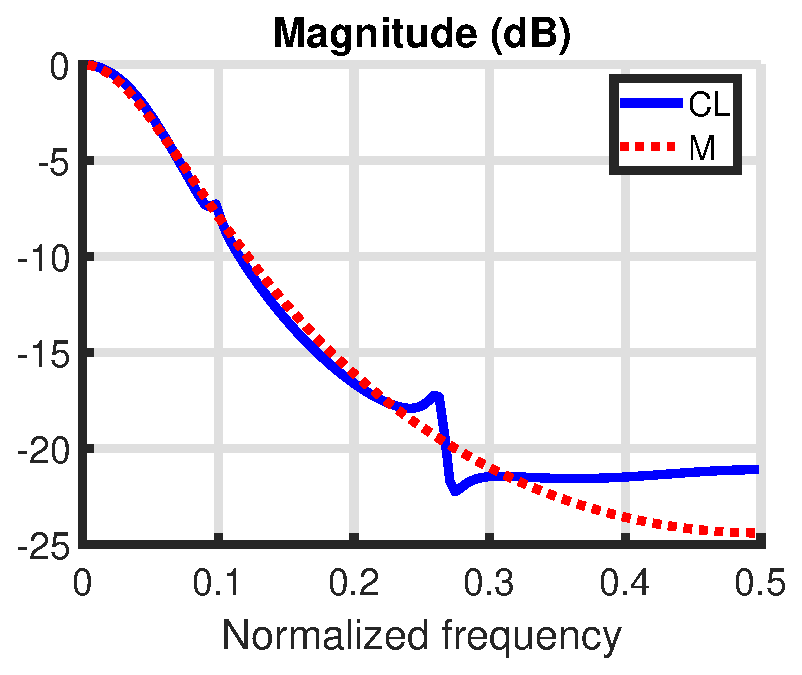
\includegraphics[width = 0.6\textwidth]{figures/undermodeled_optimal}
\caption{Reference system for the system with non realizable controller and the optimal closed loop system.}
\label{fig:non_realizable_optimal}
\end{figure}

\newpage
\paragraph{White noise}
The output is perturbed by Gaussian white noise. The results of this experiment are shown in table \ref{tab:non_realizable_white_transient_with_without_TD_vs_FD_vs_WNLS}. As expected, the optimal controller attains the best results. Notice that the cost function is not zero as the reference model is not realizable by the proposed controller structure. Note also that the convex cost $J$ (-32.49 dB) is almost equal to the original cost $J_{mr}$ (-32.48 dB). This indicates that the approximation made to attain the convex cost function is a good approximation. Additionally, the WNLS method does not perform better in this case. Moreover, the WNLS method fails when the transient is suppressed. 93 of the 100 optimizations fail when using the ``LS init'' as initial estimate. 2 of the optimizations failed when using the ``actual init'' as initial estimate. Finally, the best results are attained when using the FD method with $l_1 =  57$ without transient suppression.

\begin{table}[H]
\centering
\begin{tabular}{|ccc|}
\hline
&&\\[-2.5ex]
Method & $\Bar{J}|_{dB}$ & $\Bar{J_{mr}}|_{dB}$ \\
\hline
Optimal                                     & \textcolor{blue}{-32.49} & \textcolor{blue}{-32.48} \\
TD ($l_1 = 52$)                               & -32.30 & -32.31 \\
TD ($l_1 = 127$)                            & -32.11 & -32.13 \\
FD transient not suppressed ($l_1 = 57$)      & \textbf{-32.34} & \textbf{-32.35} \\
FD transient not suppressed ($l_1 = 254$)   & -32.08 & -32.10 \\
FD transient suppressed ($l_1 = 52$)          & -32.30 & -32.30 \\
FD transient suppressed ($l_1 = 254$)       & -31.75 & -31.78 \\
WNLS transient not suppressed (LS init)     & -31.03 & -31.01 \\
WNLS transient not suppressed (actual init) & -31.03 & -31.01 \\
WNLS transient suppressed (LS init)         & \textcolor{red}{-30.95 [93 failed]}    & \textcolor{red}{-30.93 [93 failed]}    \\
WNLS transient suppressed (actual init)     & \textcolor{red}{-30.96 [2 failed]} & \textcolor{red}{-30.93 [2 failed]} \\

\hline
\end{tabular}
\caption{System with non realizable controller with white noise. With and without transient suppression for the FD and WNLS methods. For the second, fourth and sixth rows, the parameters $l_1$ that yielded the best results are displayed.}
\label{tab:non_realizable_white_transient_with_without_TD_vs_FD_vs_WNLS}
\end{table}

\newpage
\paragraph{Coloured noise}
The same experiment is performed with coloured noise. The results are shown in table \ref{tab:non_realizable_coloured_transient_with_without_TD_vs_FD_vs_WNLS}. The optimal controller performs the best as expected. This optimal controller is available to us because we are working in simulation. Next, the WNLS method without transient suppression results in the worst controllers. 32 of the 100 optimizations failed for the WNLS method with transient suppression when using the ``LS'' init as initial estimate. 25 optimization failed when using the ``actual init'' as initial estimate. Finally, the TD method with $l_1 = 118$ performs the best. Another thing to note is that the FD method with transient suppression works better than the FD method without transient suppression. This wasn't the case when the output was perturbed with white noise (table \ref{tab:non_realizable_white_transient_with_without_TD_vs_FD_vs_WNLS}). This shows that taking the noise transients into account can give us better results.
 
\begin{table}[H]
\centering
\begin{tabular}{|ccc|}
\hline
&&\\[-2.5ex]
Method & $\Bar{J}|_{dB}$ & $\Bar{J_{mr}}|_{dB}$ \\
\hline
Optimal                                     & \textcolor{blue}{-32.4885} & \textcolor{blue}{-32.4837} \\
TD ($l_1 = 118$)                               & \textbf{-32.4709} & \textbf{-32.4676} \\
TD ($l_1 = 127$)                            & -32.4707 & -32.4675 \\
FD transient not suppressed ($l_1 = 221$)      & -32.4623 & -32.4603 \\
FD transient not suppressed ($l_1 = 254$)   & -32.4620 & -32.4602 \\
FD transient suppressed ($l_1 = 118$)          & -32.4685 & -32.4648 \\
FD transient suppressed ($l_1 = 254$)       & -32.4658 & -32.4631 \\
WNLS transient not suppressed (LS init)     & -30.3885 & -30.3817 \\
WNLS transient not suppressed (actual init) & -30.3885 & -30.3817 \\
WNLS transient suppressed (LS init)         & \textcolor{red}{-29.85 [32 failed]}      & \textcolor{red}{-29.81 [32 failed]}       \\
WNLS transient suppressed (actual init)     & \textcolor{red}{-29.72 [25 failed]}       & \textcolor{red}{-29.66 [25 failed]}       \\
\hline
\end{tabular}
\caption{System with non realizable controller with coloured noise. With and without transient suppression for the FD and WNLS methods. For the second, fourth and sixth rows, the parameters $l_1$ that yielded the best results are displayed.}
\label{tab:non_realizable_coloured_transient_with_without_TD_vs_FD_vs_WNLS}
\end{table}

% \section{Continuous time simulations}

\newpage
\section{Conclusion}
Three different methods were used to design a controller that gets the closed loop system as close as possible to a user-defined reference system $M(\Omega)$: the TD, FD and WNLS methods. The FD and WNLS methods need a nonparametric estimate of the FRF of the system $G(\Omega)$. For this nonparametric estimate the system and noise transients can be suppressed or not taken into account. Additionally, the TD and FD methods can employ the $l_1$-trick that allows for a reduction in bias.

The WNLS method with transient suppression gave the best results when the reference model $M(\Omega)$ can be realized perfectly by the proposed controller structure $K(\Omega,\rho)$. However, there is no guarantee that the optimization will converge to the global minimum. 

Applying the WNLS method when the reference cannot be realized perfectly leads to suboptimal results. In this case, the TD method usually performs better than the FD methods. When the system has a long transient and/or noise transients are present, the FD method performs better when the transient is suppressed. The FD method with transient suppression yielded the best results when the output was perturbed by white noise (table \ref{tab:non_realizable_white_transient_with_without_TD_vs_FD_vs_WNLS}, fourth row). However, when the $l_1$-trick is not used, the TD method works better than the FD method (table \ref{tab:non_realizable_white_transient_with_without_TD_vs_FD_vs_WNLS}, third and fifth rows). We mention this here because it is hard to determine which value of $l_1$ will yield the best results. In the simulations, the FRF of the system $G(\Omega)$ is known exactly, which allows us to compare all values of $l_1$. Thus, when working with real measurements, one would probably just use the maximum value of $l_1$ unless one has some prior knowledge of the system.

Thus we can conclude that the TD method works the best on DT systems, unless the reference model is realizable. If the reference model is realizable, then the WNLS method performs the best. Note however, that the TD method only works on DT systems. If one wants to design an analog controller for a CT system, the TD method will not work. In this sense, the proposed FD method is more general than the TD method.
